\documentclass[conference]{IEEEtran}
\IEEEoverridecommandlockouts

\usepackage{cite}
\usepackage{amsmath,amssymb,amsfonts}
\usepackage{graphicx}
\usepackage{textcomp}
\usepackage{xcolor}
\usepackage{booktabs}
\usepackage{url}

\newcommand{\pp}{\,pp}
\graphicspath{{figures/}}

\begin{document}

\title{Pruning and Int8 Quantization for CNN Inference on a Cortex-M7 Microcontroller: A Controlled Multi-Seed Study}

\author{\IEEEauthorblockN{Yerman Bekzat}
\IEEEauthorblockA{\textit{Department (to be completed)} \\
\textit{University (to be completed)}\\
City, Country \\
yermanbekzat@gmail.com}
}

\maketitle

\begin{abstract}
Reported gains from quantization and pruning on embedded hardware are hard to compare: studies differ in models, platforms and metrics, and often report energy or latency without a matching accuracy analysis. We present a controlled comparison under one fixed, pre-registered protocol. MobileNetV2 trained on CIFAR-10 is pruned structurally at 0, 25, 50 and 75 percent of its channels and quantized to int8 with post-training quantization and quantization-aware training, giving 48 models over three random seeds. Accuracy is measured on the exported models and latency and memory on an STM32H7B3 microcontroller running at 280 MHz. Int8 quantization alone reduces latency and estimated energy by 4.2 times at a cost of 1.6 percentage points of accuracy; adding 25 percent pruning raises the saving to 5.1 times at a cost of 3.6 points. No compressed configuration meets the pre-registered budget of 1 point. Quantization-aware training beats post-training quantization by 0.4 points on average, and its advantage grows with the pruning ratio. Multiply-accumulate counts rank latency correctly within one numeric precision but not across precisions. At 50 to 75 percent pruning, int8 accuracy varies by up to 33 points across seeds, against at most 2.3 points for full-precision models, so single-seed results can misrepresent aggressive compression. Code, logs and results are public.
\end{abstract}

\begin{IEEEkeywords}
TinyML, quantization, structured pruning, microcontrollers, energy efficiency, benchmarking
\end{IEEEkeywords}

\section{Introduction}
Running convolutional neural networks (CNNs) on the device that collects the data removes the latency and energy cost of sending it to the cloud~\cite{verhelst2020edge}. On microcontrollers the obstacle is size: even compact CNNs need millions of multiply-accumulate operations (MACs) and hundreds of kilobytes of memory. Quantization and pruning are the two main levers for closing that gap~\cite{han2016deep,jacob2018quantization}, often combined with hardware--software co-design~\cite{chen2017eyeriss,hao2020codesign,yang2019synetgy}.

The evidence on how far these levers go is hard to use. In a review of the literature on energy-efficient CNN acceleration for embedded systems we found three recurring problems. First, studies use different datasets, platforms and metrics, so their figures cannot be compared~\cite{peccia2024gemmini,blalock2020state}. Second, energy and latency gains are often reported without a rigorous account of the accuracy lost~\cite{chung2025depthwise}; reports even disagree on whether int8 quantization costs accuracy at all~\cite{choi2022efficient,chung2025depthwise}. Third, techniques are often evaluated without modeling memory bandwidth and resource limits, so gains estimated from proxies such as operation counts may not appear on a real device~\cite{choi2022efficient,yang2017energy}.

This paper addresses these problems with a small, controlled study in which only the compression settings change. Its contributions are:
\begin{itemize}
\item A fixed protocol: one model, one dataset, one microcontroller and one measurement procedure, with the plan, hypotheses and selection rule committed before any experiment and every deviation logged.
\item A full factorial comparison of structured pruning (four ratios) and int8 quantization (post-training and quantization-aware) over three seeds, 48 models in total, with accuracy measured on the deployed model files and latency and memory measured on an STM32H7B3 board.
\item Three findings for practitioners and reviewers: int8 dominates pruning alone on the accuracy--energy front; MAC counts mislead across numeric precisions; and int8 accuracy after aggressive pruning varies so much across seeds that single-seed reports are unreliable.
\item An open archive of code, configurations, raw device logs and results~\cite{repo}.
\end{itemize}

\section{Related Work}
\textit{Quantization.} Integer-only int8 inference with per-channel weights and per-tensor activations is the standard deployment path for CNNs~\cite{jacob2018quantization,krishnamoorthi2018whitepaper}. On microcontrollers, mixed low-precision schemes fit larger networks into memory~\cite{rusci2020memory}, and instruction-set extensions speed up quantized kernels on RISC-V cores~\cite{garofalo2020xpulpnn}. Depthwise-separable networks such as MobileNet are known to be sensitive to per-tensor quantization because channel ranges differ widely~\cite{krishnamoorthi2018whitepaper,nagel2019dfq}, and quantization combined with fast convolution algorithms can be numerically unstable~\cite{mori2024wino}.

\textit{Pruning.} Pruning moved from removing individual weights by magnitude~\cite{han2015learning} to removing whole filters by their norm~\cite{li2017pruning} and to energy-aware selection~\cite{yang2017energy}. Structured pruning yields a smaller dense network that any hardware can run faster, whereas unstructured sparsity needs dedicated support. Dependency-aware tools now prune architectures with residual connections automatically~\cite{fang2023depgraph}. Pruning and quantization have been combined since Deep Compression~\cite{han2016deep}.

\textit{Embedded deployment and benchmarking.} Optimized kernels such as CMSIS-NN make int8 inference practical on Cortex-M cores~\cite{lai2018cmsisnn}, and MLPerf Tiny defines a common benchmark for such devices~\cite{banbury2021mlperftiny}. Accelerator studies cut energy on ASICs and FPGAs, mainly by reducing data movement~\cite{chen2017eyeriss,peccia2024gemmini}; approximate computing trades accuracy for energy~\cite{moons2016energy}, and adaptive schemes tune that trade-off at run time~\cite{jayakodi2018trading,hemmat2021airnn}. Critiques of the pruning literature point to inconsistent baselines and metrics~\cite{blalock2020state}, and work on benchmark variance shows that ignoring seed-to-seed variation can lead to wrong conclusions~\cite{bouthillier2021variance}. Our study applies these lessons to compression on a real microcontroller.

\section{Method}

\subsection{Design and hypotheses}
The study crosses pruning ratio (0, 25, 50, 75\,\% of channels) with numeric format (fp32, int8 post-training quantization (PTQ), int8 quantization-aware training (QAT)), each trained with seeds 1--3. Model, data, training recipe, board and measurement are fixed. The plan stated three hypotheses: H1, pruning combined with int8 dominates either technique alone on the accuracy--energy Pareto front; H2, QAT loses less accuracy than PTQ, and more so at high pruning; H3, MAC count preserves the ranking of configurations by measured latency (Spearman $\rho \geq 0.8$). It also fixed a selection rule: the best configuration is the one with the lowest energy whose mean accuracy is within 1\pp\ of the fp32 baseline.

\subsection{Model and training}
We use MobileNetV2~\cite{sandler2018mobilenetv2} with width multiplier 0.35 on CIFAR-10~\cite{krizhevsky2009cifar}. For $32\times32$ inputs the first convolution and the first stride-2 depthwise convolution use stride 1, so the last feature map is $4\times4$. The baseline has 408{,}938 parameters and 17.6\,M MACs. Each seed trains its own baseline in PyTorch~\cite{paszke2019pytorch} for 100 epochs with SGD (Nesterov momentum 0.9, learning rate 0.05 with cosine decay, weight decay $4\times10^{-5}$, batch 128), random crops and horizontal flips.

\subsection{Structured pruning}
Channels are removed with Torch-Pruning~\cite{fang2023depgraph}, which keeps channels coupled by residual connections consistent. Importance is the L1 norm of each channel's weights~\cite{li2017pruning}; the same ratio is applied to every layer except the classifier, so all seeds of a ratio share one architecture (Table~\ref{tab:hw}). Each pruned model is fine-tuned for 15 epochs (learning rate 0.01, cosine decay).

\subsection{Quantization}
Models are exported to ONNX (opset 13, batch normalization folded) and quantized with ONNX Runtime~\cite{onnxruntime} static quantization in QDQ format: int8 weights, symmetric per channel; int8 activations, asymmetric per tensor; 500 fixed calibration images. The activation calibration method was chosen on a validation split of 5{,}000 training images disjoint from the calibration set, never on the test set. Candidates were min--max and percentile calibration (99.999, 99.99, 99.9); the fixed rule picks the smallest mean accuracy drop over the 12 fp32 models, with ties within 0.1\pp\ going to the simpler method. Percentile 99.99 won with a mean drop of 6.71\pp\ against 7.96\pp\ for min--max; min--max was as good at 0--25\,\% pruning, and the difference arose at 50--75\,\% (11.27 vs.\ 6.77\pp\ at 50\,\%).

For QAT, batch normalization is folded into the convolutions and training rounds weights (per channel) and activations (after each ReLU6, after each block's projection convolution and after each residual addition) to int8 in the forward pass with a straight-through gradient. Activation ranges are computed on the same 500 calibration images with the same percentile rule and refreshed before every epoch, so training sees the ranges the deployed model will receive. Afterwards the weights are left on the int8 grid and the model passes through the same quantizer as PTQ; PTQ and QAT models therefore have identical graphs and differ only in weight values. QAT uses learning rate 0.001 with cosine decay for 5 epochs (QAT-5, pre-registered). As a sensitivity check we added 15 epochs (QAT-15), the budget of the pruning fine-tune, both starting from the same fp32 model.

\subsection{Hardware and metrics}
Latency and memory are measured on an STM32H7B3I-DK board (Cortex-M7, 280\,MHz, 2\,MB Flash, 1.4\,MB RAM) through ST Edge AI Developer Cloud with ST Edge AI Core 4.1.0~\cite{stedgeai}. The models are uploaded already quantized. The code-generation objective is Balanced, except for the 25\,\% int8 models, which only link with the RAM objective. Weights reside in internal Flash and activations in internal RAM for every model. Latency is the on-device duration of one inference; Flash is weights plus runtime, RAM is activations plus runtime. ST's validation compares the board output with the ONNX model on a random input: cosine similarity is 1.0 for all models but one (0.9987, 75\,\% QAT).

Seeds change weight values but not layer sizes, so seed-1 models represent each architecture on the board. PTQ and QAT latencies agree within 0.1\,\%, and int8 uses their mean. Energy per inference is $E = P\,t$ with $P = 3.3\,\text{V} \times 120\,\mu\text{A/MHz} \times 280\,\text{MHz} = 110.9$\,mW, the typical run-mode figure for this device~\cite{stm32h7b3}. It is an estimate for the microcontroller alone and is proportional to latency. Accuracy is top-1 on the 10{,}000 CIFAR-10 test images, computed with ONNX Runtime on the exported file.

\subsection{Statistics}
We report mean $\pm$ standard deviation over seeds. For H2, differences are paired by pruning ratio and seed; we give 95\,\% $t$-intervals per ratio and, over all 12 pairs, a one-sided Wilcoxon signed-rank test and a Spearman correlation with the pruning ratio. H3 uses Spearman's $\rho$ over the eight distinct architectures.

\subsection{Deviations from the plan}
All deviations are dated in the project log~\cite{repo}. (i) The planned NUCLEO-H743ZI2 board could not link the fp32 baseline, because its benchmark firmware places activations in 128\,KB of tightly coupled memory; an STM32N6 board was rejected because it has a neural accelerator and no internal Flash. (ii) A first run used min--max calibration, and QAT used moving-average ranges discarded at export. Int8 accuracy collapsed at 50--75\,\% pruning, and QAT was no better than PTQ. We replaced both with the procedures above and archived the first run. (iii) QAT-15 was added as a sensitivity analysis; QAT-5 remains the pre-registered result. (iv) The 25\,\% int8 models use the RAM objective.

\section{Results}

\subsection{Accuracy and hardware cost}
Table~\ref{tab:acc} gives accuracy for all 48 models and Table~\ref{tab:hw} the measured cost of each architecture. Int8 cuts latency 3.4--4.3$\times$ at every pruning ratio and Flash 1.9--3.4$\times$; the Flash saving shrinks for small models because the runtime code is a fixed cost. The smallest model, int8 at 75\,\%, needs 79\,KB of Flash and 35\,KB of RAM, against 1{,}591\,KB and 273\,KB for the baseline. Int8 costs 1.6--1.8\pp\ of accuracy at 0--25\,\% pruning but 6.6\pp\ at 50\,\% and 15.0\pp\ at 75\,\% (PTQ).

\begin{table}[t]
\caption{Top-1 accuracy (\%), mean $\pm$ std over 3 seeds}
\label{tab:acc}
\centering
\setlength{\tabcolsep}{4pt}
\begin{tabular}{@{}lcccc@{}}
\toprule
Pruned & fp32 & PTQ & QAT-5 & QAT-15 \\
\midrule
0\,\%  & $89.49 \pm 0.13$ & $87.88 \pm 0.68$ & $87.71 \pm 0.88$ & $87.94 \pm 0.65$ \\
25\,\% & $87.60 \pm 0.43$ & $85.81 \pm 0.81$ & $85.88 \pm 0.74$ & $86.08 \pm 0.73$ \\
50\,\% & $81.64 \pm 0.15$ & $75.00 \pm 5.92$ & $75.66 \pm 6.00$ & $77.14 \pm 4.67$ \\
75\,\% & $66.97 \pm 1.21$ & $52.01 \pm 17.75$ & $53.19 \pm 16.88$ & $54.14 \pm 15.45$ \\
\bottomrule
\end{tabular}
\end{table}

\begin{table}[t]
\caption{Measured cost per architecture on STM32H7B3 (280\,MHz). Energy is estimated as 110.9\,mW $\times$ latency}
\label{tab:hw}
\centering
\setlength{\tabcolsep}{3.2pt}
\begin{tabular}{@{}lrrlrrrr@{}}
\toprule
Pruned & Params & MACs & Format & Latency & Flash & RAM & Energy \\
 & & (M) & & (ms) & (KB) & (KB) & (mJ) \\
\midrule
0\,\%  & 408{,}938 & 17.55 & fp32 & 427.2 & 1{,}591 & 273 & 47.36 \\
       &           &       & int8 & 100.5 &   475 & 137 & 11.14 \\
25\,\% & 239{,}554 & 10.77 & fp32 & 289.9 &   936 & 221 & 32.15 \\
       &           &       & int8 &  84.2 &   297 &  84 &  9.33 \\
50\,\% & 114{,}938 &  5.58 & fp32 & 165.4 &   457 & 151 & 18.34 \\
       &           &       & int8 &  42.3 &   167 &  42 &  4.69 \\
75\,\% &  35{,}090 &  1.99 & fp32 &  70.0 &   151 & 115 &  7.77 \\
       &           &       & int8 &  20.2 &    79 &  35 &  2.24 \\
\bottomrule
\end{tabular}
\end{table}

\subsection{Pareto front and selection}
Fig.~\ref{fig:pareto} plots accuracy against energy. Among the pre-registered variants, the front consists of the fp32 baseline, int8 PTQ at 0\,\%, and int8 QAT-5 at 25, 50 and 75\,\%. No compressed configuration meets the 1\pp\ rule, because int8 at 0\,\% already loses 1.61\pp; by the rule, the uncompressed baseline is selected. Table~\ref{tab:sel} shows the best choice at looser budgets: int8 alone saves 4.2$\times$ energy within 2\pp, and adding 25\,\% pruning saves 5.1$\times$ within 5\pp. Including QAT-15 picks the same architectures with 0.1--1.5\pp\ higher accuracy.

\begin{figure}[t]
\centering
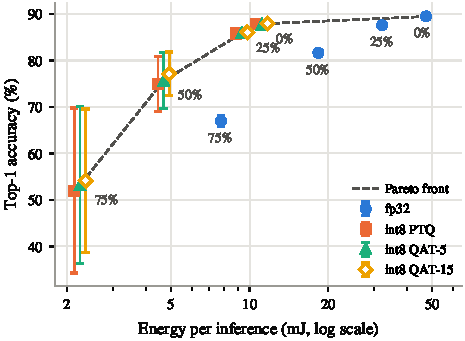
\includegraphics[width=\columnwidth]{pareto}
\caption{Accuracy vs.\ estimated energy per inference (mean $\pm$ std, 3 seeds; labels give the pruning ratio). Int8 variants share one energy value per ratio and are offset horizontally for legibility. The dashed line is the Pareto front of the pre-registered variants.}
\label{fig:pareto}
\end{figure}

\begin{table}[t]
\caption{Lowest-energy configuration within an accuracy budget (pre-registered variants)}
\label{tab:sel}
\centering
\setlength{\tabcolsep}{4pt}
\begin{tabular}{@{}rllrrr@{}}
\toprule
Budget & Pruned & Variant & Acc. (\%) & Energy (mJ) & Saving \\
\midrule
1\pp  & 0\,\%  & fp32       & 89.49 & 47.36 & 1.0$\times$ \\
2\pp  & 0\,\%  & int8 PTQ   & 87.88 & 11.14 & 4.2$\times$ \\
5\pp  & 25\,\% & int8 QAT-5 & 85.88 &  9.33 & 5.1$\times$ \\
15\pp & 50\,\% & int8 QAT-5 & 75.66 &  4.69 & 10.1$\times$ \\
\bottomrule
\end{tabular}
\end{table}

\subsection{H1: combined compression}
All three pruning-only (fp32) points lie off the front: two are dominated by combined configurations and the 25\,\% point by int8 alone. For example, fp32 at 75\,\% reaches 66.97\,\% at 7.77\,mJ, while int8 at 50\,\% reaches 75.66\,\% at 4.69\,mJ. Combined configurations extend the front below 11\,mJ but do not dominate int8 at 0\,\%, which remains the most accurate low-energy point. H1 therefore holds against pruning alone but not against quantization alone.

\subsection{H2: QAT versus PTQ}
Fig.~\ref{fig:qat} shows the accuracy gain of QAT over PTQ for each model. QAT-5 beats PTQ in 9 of 12 pairs by $+0.43$\pp\ on average (95\,\% CI $[-0.03, +0.90]$; Wilcoxon $p = 0.026$), and the gain grows with pruning ($\rho = 0.84$, $p = 0.001$): from $-0.17$\pp\ at 0\,\% to $+1.17$\pp\ at 75\,\%. QAT-15 raises the mean gain to $+1.15$\pp\ (CI $[+0.16, +2.14]$; 11 of 12 positive; $p < 0.001$), reaching $+2.1$\pp\ at 50 and 75\,\%. QAT-15 beats QAT-5 by $+0.72$\pp\ (CI $[+0.07, +1.36]$, $p = 0.001$). With three seeds the per-ratio intervals all include zero; the 12-pair test carries the evidence. H2 is supported, but QAT does not rescue the two most degraded models (next subsection).

\begin{figure}[t]
\centering
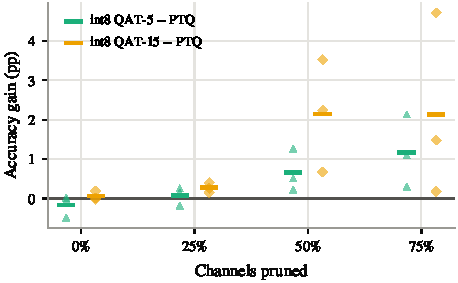
\includegraphics[width=\columnwidth]{qat_gain}
\caption{Accuracy gain of QAT over PTQ, paired by model. Markers: individual seeds; bars: means.}
\label{fig:qat}
\end{figure}

\subsection{H3: MACs as a latency proxy}
Across the eight architectures, MACs and latency correlate with $\rho = 0.73$ ($p = 0.039$), below the 0.8 threshold, so H3 is not supported. Within one precision the ranking is perfect ($\rho = 1.0$ for fp32 and for int8; Fig.~\ref{fig:macs}), but across precisions it fails: int8 at 0\,\% performs 17.6\,M MACs in 100.5\,ms, whereas fp32 at 50\,\% performs only 5.6\,M MACs and takes 165.4\,ms. Cost per MAC also rises as layers narrow, from 24.3 to 35.2\,ns for fp32 and from 5.7 to 10.2\,ns for int8, so pruning 25\,\% of int8 channels removes 39\,\% of MACs but only 16\,\% of latency.

\begin{figure}[t]
\centering
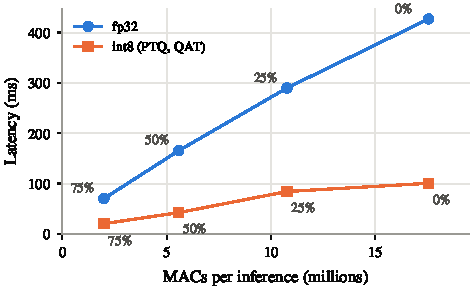
\includegraphics[width=\columnwidth]{macs_latency}
\caption{MAC count vs.\ measured latency. Labels give the pruning ratio.}
\label{fig:macs}
\end{figure}

\subsection{Seed sensitivity}
Fig.~\ref{fig:seeds} shows every model. Full-precision accuracy varies by at most 2.3\pp\ across seeds, but int8 accuracy after aggressive pruning varies widely: 68.2--79.2\,\% at 50\,\% (PTQ) and 31.7--64.4\,\% at 75\,\%. The spread comes from two models. At 75\,\% with seed 1, int8 falls from 66.0\,\% to 31.7\,\% (PTQ), 33.8\,\% (QAT-5) and 36.4\,\% (QAT-15), while seed 3 loses about 2\pp. At 50\,\% with seed 2, accuracy falls from 81.7\,\% to 68.2--71.8\,\%. No calibration method rescues them: in the validation study their best-case drops were 25.7\pp\ and 12.5\pp. The sensitivity belongs to these model instances, not to the pipeline, which is identical across seeds.

\begin{figure}[t]
\centering
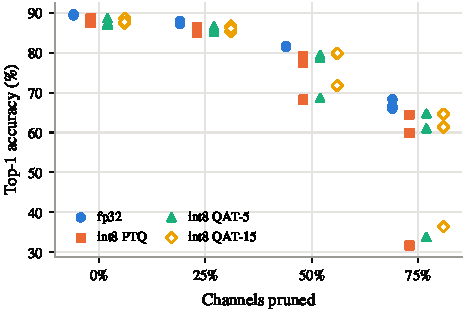
\includegraphics[width=\columnwidth]{seeds}
\caption{Accuracy of all 48 models, one marker per seed.}
\label{fig:seeds}
\end{figure}

\section{Discussion}
\textit{Practical guidance.} For this model and device, int8 quantization should come first: it is the largest and cheapest saving, 4.2$\times$ energy and 3.3$\times$ Flash for 1.6\pp. Structured pruning adds less. The network is already narrow at width 0.35, so accuracy drops quickly, and the measured speed-up lags the reduction in MACs because narrow layers use the kernels less efficiently. Pruning 25\,\% on top of int8 is a reasonable step; going further trades accuracy steeply for modest additional savings.

\textit{Reporting.} Two results bear on how compression results should be reported. First, MAC counts are a valid proxy only within one numeric precision; any comparison across fp32 and int8 needs measurement on the target. Second, a single seed could have reported 64\,\% or 32\,\% for the same 75\,\% int8 configuration. Studies of aggressive compression should report several seeds and the accuracy of every deployed model, not only a mean or the best run~\cite{bouthillier2021variance}. This supports the call in our review for mandatory, rigorous accuracy reporting alongside efficiency gains.

\textit{Why some models collapse.} We did not identify the layer responsible. A plausible cause is the per-tensor activation quantization of depthwise layers whose channel ranges differ widely, a known weakness of MobileNet-style networks~\cite{krishnamoorthi2018whitepaper,nagel2019dfq} that pruning may amplify. Per-layer error analysis and cross-layer equalization~\cite{nagel2019dfq} are natural next steps.

\textit{Limitations.} The study covers one model, one dataset and one microcontroller; CIFAR-10 and a small MobileNetV2 limit how far the conclusions generalize. Energy is estimated from a datasheet figure for the microcontroller alone, not measured, and therefore mirrors latency; board-level power measurement would capture memory-access effects. Three seeds give wide per-ratio intervals. The 25\,\% int8 models used a different code-generation objective, the ST runtime chose memory placement per model, and one model showed a small numerical mismatch between board and reference. Accuracy was measured with ONNX Runtime rather than on the board.

\section{Conclusion}
Under one fixed protocol on an STM32H7B3 microcontroller, int8 quantization dominated structured pruning alone, saving 4.2$\times$ estimated energy for 1.6\pp\ of accuracy. Combining it with 25\,\% pruning raised the saving to 5.1$\times$ for 3.6\pp, but no compressed configuration met a 1\pp\ budget. QAT recovered a small and significant amount of accuracy over PTQ, growing with the pruning ratio. MAC counts failed as a latency proxy across precisions, and int8 accuracy after aggressive pruning varied by up to 33\pp\ between seeds. Compression studies for microcontrollers should therefore measure on the target and report results over several seeds. Code, configurations, raw device logs and results are available at~\cite{repo}.

\bibliographystyle{IEEEtran}
\bibliography{references}

\end{document}
